\chapter{Rantai Makanan}\label{ch:g3:food-chains}

Rumput tumbuh di padang rumput. Seekor belalang memakan rumputnya.
Seekor kadal menangkap belalangnya. Seekor elang, yang berputar tinggi
di udara, menyambar kadalnya. Empat santapan --- dan tiba-tiba sore
hari sang elang bergantung pada sehijau apa rumputnya tumbuh. Santapan
di alam bersambung menjadi rantai, dan belajar membacanya berarti
belajar bagaimana seluruh padang rumput bertahan bersama.

\section{Membaca dan menuliskan sebuah rantai makanan}

\begin{definition}[Rantai makanan]\label{def:g3:food-chains:chain}
Suatu \emph{rantai makanan}\index{rantai makanan} adalah barisan
\omterm{def:g1:living-or-not:living}{makhluk hidup} yang masing-masingnya dimakan oleh yang berikutnya. Ia
dituliskan dengan anak panah, tiap anak panah berarti \emph{``dimakan
oleh''}\index{dimakan oleh}:
\[
\text{rumput} \longrightarrow \text{belalang}
\longrightarrow \text{kadal} \longrightarrow \text{elang}.
\]
Tiap \omterm{def:g1:living-or-not:living}{makhluk hidup} adalah sebuah \emph{mata rantai}\index{mata rantai}
dari rantainya.
\end{definition}

\begin{remark}[Perhatikan arah anak panahnya]\label{rem:g3:food-chains:arrow}
Anak panahnya menunjuk dari yang dimakan ke yang memakan --- ia
mengikuti makanannya. ``Rumput $\rightarrow$ belalang'' dibaca
``rumput \omterm{def:g3:food-chains:chain}{dimakan oleh} belalang''. Menuliskan anak panahnya terbalik
--- ke arah santapannya --- adalah kekeliruan yang paling sering
terjadi pada \omterm{def:g3:food-chains:chain}{rantai makanan}; ingatlah bahwa anak panahnya menunjukkan
ke mana makanannya \emph{pergi}.
\end{remark}

\begin{proposition}[Setiap rantai bermula pada tumbuhan]\label{prop:g3:food-chains:start}
Mata rantai pertama sebuah \omterm{def:g3:food-chains:chain}{rantai makanan} selalu berupa \omterm{def:g1:plants-around-us:plant}{tumbuhan} (atau
\omterm{def:g1:living-or-not:living}{makhluk hidup} lain yang membuat makanannya sendiri). Hanya \omterm{def:g1:plants-around-us:plant}{tumbuhan}
yang makan tanpa memakan siapa pun --- dari cahaya, air dan udara,
seperti dikatakan \cref{def:g1:plants-around-us:plant}. Setiap mata
rantai \omterm{def:g1:animals-around-us:animal}{hewan} hidup, langsung atau melalui yang lain, dari mata rantai
hijau yang pertama itu.
\end{proposition}
\admitted

\begin{example}[Rantai dari tiga habitat]\label{ex:g3:food-chains:three}
Di kolam: \omterm{def:g1:plants-around-us:plant}{tumbuhan} air $\rightarrow$ \omterm{ex:g2:animals-grow-up:frog}{berudu} $\rightarrow$ larva capung
$\rightarrow$ \omterm{prop:g3:sorting-living-things:groups}{ikan} duri $\rightarrow$ kuntul. Di hutan: \omterm{def:g1:plants-around-us:parts}{daun} pohon ek
$\rightarrow$ \omterm{ex:g2:animals-grow-up:butterfly}{ulat} $\rightarrow$ \omterm{prop:g3:sorting-living-things:groups}{burung} gelatik biru $\rightarrow$
alap-alap. Di kebun: selada $\rightarrow$ siput $\rightarrow$ landak.
Mata rantai pertama: selalu hijau.
\end{example}

\begin{omfigure}
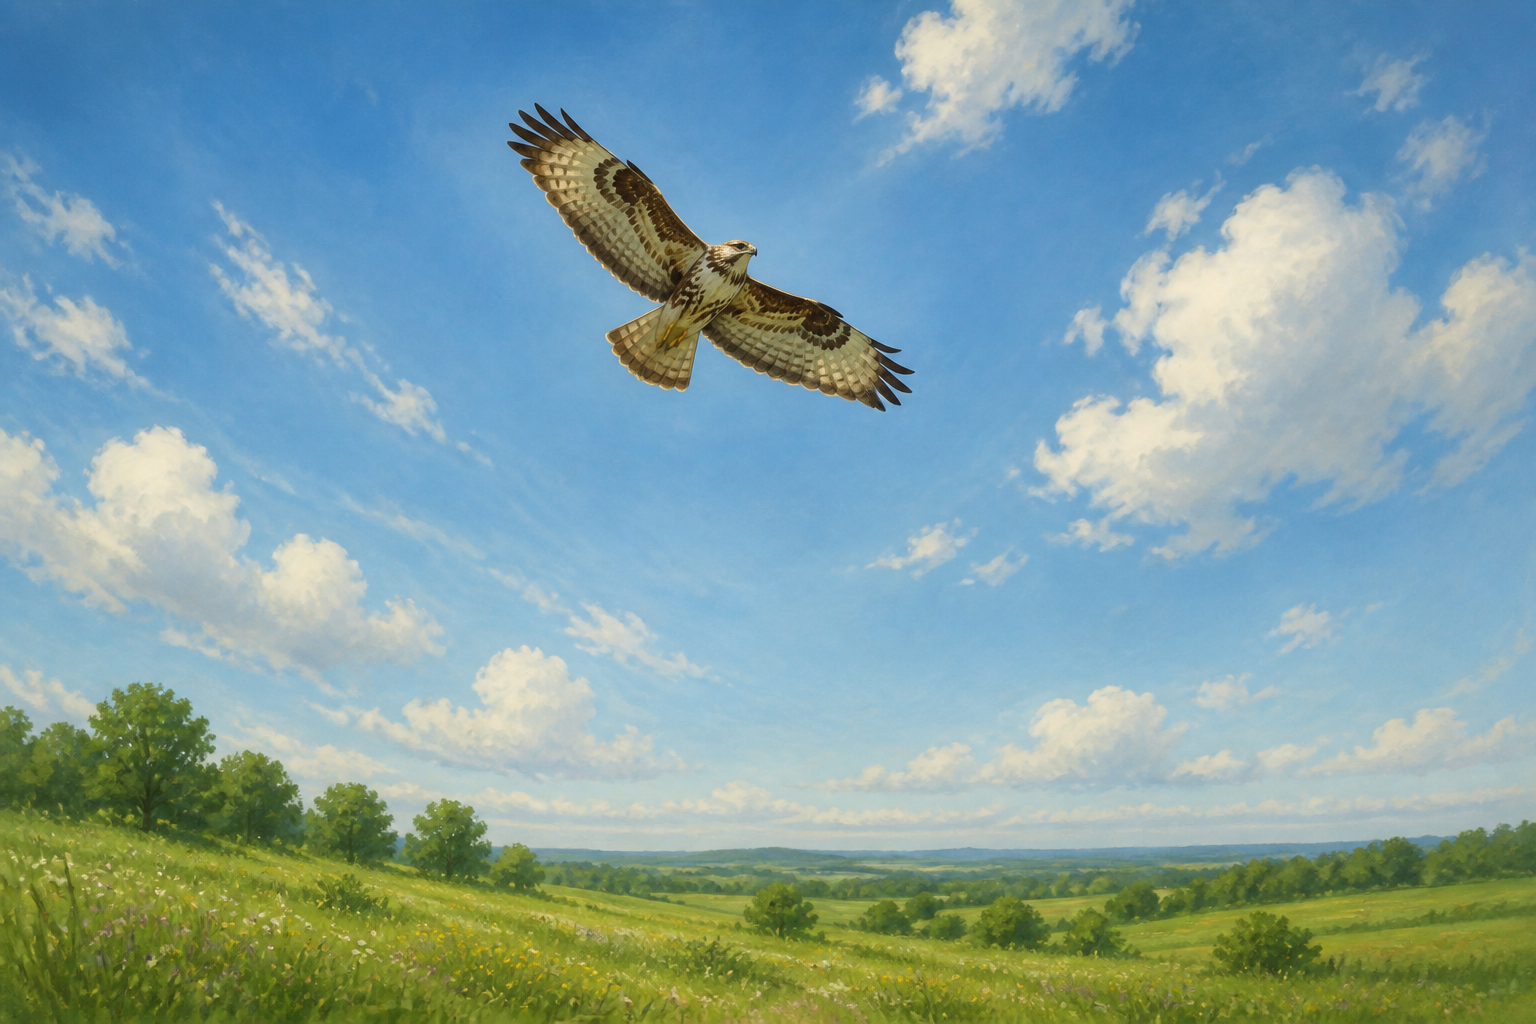
\includegraphics[width=0.6\linewidth]{images/book1/ai/g3-chains-buzzard.png}

{\small Mata rantai terakhir rantai padang rumputnya sedang
berpatroli: sore hari sang elang bergantung, tiga mata rantai di
bawahnya, pada sehijau apa rumputnya tumbuh.}
\end{omfigure}

\begin{method}[Menyusun sebuah rantai makanan]\label{met:g3:food-chains:build}
\begin{enumerate}
  \item Pilih seekor \omterm{def:g1:animals-around-us:animal}{hewan} lalu tanyakan: apa yang dimakannya?
        Tuliskan makanannya di sebelah kirinya, anak panah menunjuk ke
        yang memakan;
  \item ajukan pertanyaan yang sama tentang makanannya, dan lanjutkan
        ke kiri sampai kamu sampai pada sebuah \omterm{def:g1:plants-around-us:plant}{tumbuhan};
  \item tanyakan: siapa yang memakan \omterm{def:g1:animals-around-us:animal}{hewan} awalku? Perpanjang ke kanan
        selama masih ada yang memakannya;
  \item periksa bahwa setiap anak panah terbaca \omterm{def:g3:food-chains:chain}{``dimakan oleh''} ---
        makanan mengalir ke kanan.
\end{enumerate}
\end{method}

\section{Ketika sebuah mata rantai berubah}

\begin{proposition}[Mata rantai saling bergantung]\label{prop:g3:food-chains:depend}
Dalam sebuah \omterm{def:g3:food-chains:chain}{rantai makanan}, setiap mata rantai bergantung pada yang
mendahuluinya, dan memberi makan yang sesudahnya. Kalau satu mata
rantai menjadi langka, mata rantai berikutnya kelaparan --- dan mata
rantai \emph{sebelumnya}, yang tidak lagi dimakan sebanyak itu, dapat
berlipat ganda. Sebuah perubahan pada satu mata rantai merambat
sepanjang seluruh rantainya.
\end{proposition}
\admitted

\begin{example}[Musim panas yang kering]\label{ex:g3:food-chains:dry}
Kemarau panjang mencokelatkan rumput padang rumputnya. Belalang, yang
kekurangan makanan, menjadi sedikit; kadal yang memburunya kelaparan
lalu memberi makan elangnya dengan buruk pada gilirannya. Satu mata
rantai pertama yang mencokelat, dan seluruh rantai di atasnya menipis
--- elangnya tidak pernah memakan rumput, namun ia merasakan
kemaraunya.
\end{example}

\begin{example}[Menyingkirkan pemburunya]\label{ex:g3:food-chains:hunter}
Andaikan elang-elangnya lenyap dari lembahnya. Kadal, yang lebih
sedikit diburu, berlipat ganda; belalang lalu dimakan lebih keras dan
menyusut; rumputnya, yang lebih sedikit dikunyah, bahkan dapat
menebal. Menyingkirkan mata rantai yang \emph{terakhir} pun merambat
sepanjang rantainya --- ke arah yang sebaliknya.
\end{example}

\begin{remark}[Padang rumput yang sesungguhnya berupa jaring]\label{rem:g3:food-chains:web}
Rantai kita adalah satu utas benang, tetapi elangnya juga menyambar
tikus, kadalnya juga memakan lalat, dan rumputnya memberi makan
kelinci pula. Banyak rantai yang bersilangan membentuk sebuah jala ---
yaitu \emph{jaring makanan} yang akan dipelajari pada tahun berikutnya
(\cref{ch:g2:what-animals-eat} sudah mengisyaratkannya dengan rubah,
kelinci dan rumput). Rantai lebih dahulu: rantailah benang yang
menganyam jalanya.
\end{remark}

\section{Latihan}

\begin{exercise}[$\star$]\label{exo:g3:food-chains:1}
Apa arti anak panah pada sebuah \omterm{def:g3:food-chains:chain}{rantai makanan}? Ke arah mana ia
menunjuk?
\end{exercise}

\begin{exercise}[$\star$]\label{exo:g3:food-chains:2}
\omterm{def:g1:living-or-not:living}{Makhluk hidup} jenis apa yang selalu menjadi mata rantai pertama?
Mengapa?
\end{exercise}

\begin{exercise}[$\star$]\label{exo:g3:food-chains:3}
Tuliskan rantai padang rumput dalam bab ini dengan keempat mata
rantainya dan anak panahnya.
\end{exercise}

\begin{exercise}[$\star$]\label{exo:g3:food-chains:4}
Betulkan rantai berikut: rubah $\rightarrow$ kelinci $\rightarrow$
rumput.
\end{exercise}

\begin{exercise}[$\star$]\label{exo:g3:food-chains:5}
Susunlah sebuah rantai dari mata rantai berikut: \omterm{prop:g3:sorting-living-things:groups}{burung} gelatik biru,
\omterm{def:g1:plants-around-us:parts}{daun} pohon ek, alap-alap, \omterm{ex:g2:animals-grow-up:butterfly}{ulat}.
\end{exercise}

\begin{exercise}[$\star$]\label{exo:g3:food-chains:6}
Pada rantai kebun selada $\rightarrow$ siput $\rightarrow$ landak,
siapa yang dimakan siputnya? Siapa yang memakan siputnya?
\end{exercise}

\begin{exercise}[$\star$]\label{exo:g3:food-chains:7}
Pakai \cref{met:g3:food-chains:build} untuk membuat sebuah rantai
sedikitnya tiga mata rantai yang berakhir dengan kuntul di kolamnya.
\end{exercise}

\begin{exercise}[$\star$]\label{exo:g3:food-chains:8}
Pada musim panas yang kering \cref{ex:g3:food-chains:dry}, mengapa
elangnya menderita walaupun ia tidak pernah memakan rumput?
\end{exercise}

\begin{exercise}[$\star\star$]\label{exo:g3:food-chains:9}
Tukang kebun yang meracuni setiap siput kadang kehilangan landaknya
--- lalu kemudian berjumpa siput telanjang dan siput \emph{lebih
banyak} daripada sebelumnya. Jelaskan kedua paruhnya dengan
\cref{prop:g3:food-chains:depend}.
\end{exercise}

\begin{exercise}[$\star\star$]\label{exo:g3:food-chains:10}
``Kadalnya bergantung pada rumputnya.'' Benar atau salah? Belalah
jawabanmu dengan rantai padang rumputnya --- lalu sebutkan ke arah
mana kegagalan rumputnya merambat.
\end{exercise}
